\newpage

\section{Выполнение лабораторной работы} 

\subsection{Описание выбранного датасета}

\begin{itemize}
    \item Название датасета: Iris — размеры цветков ириса
\item Описание: измерения размеров трёх видов растений ирисов
\item Количество наблюдений: 150
\item Количество признаков: 4
\item Тип признаков: количественные
\item Шкалы измерений: номинальная, отношений
\item Наличие пропусков: 0
\end{itemize}

\subsection{Методика исследования}

Часть 1: Подготовка и первичный осмотр данных

\begin{enumerate}
    \item Загрузка данных в pandas.DataFrame
\item Вывод размерности, типов данных, первых и последних строк
\item Проверка пропусков и дубликатов
\item Определение типа и шкалы измерений для каждого признака
\item Анализ корректности вычисления среднего для каждого признака
\end{enumerate}

Часть 2: Проверка базовых предположений (4-Plot)
\begin{enumerate}
    \item Построение Run Sequence Plot
    \item Построение Lag Plot
    \item Построение гистограммы
    \item Построение Normal Probability Plot
    \item Интерпретация каждого графика и вывод о выполнении предположений
\end{enumerate}


Часть 3: Описательная статистика
\begin{enumerate}
    \item Расчёт мер центральной тенденции: среднее, медиана, мода
    \item Расчёт мер разброса: дисперсия, стандартное отклонение, IQR, MAD, размах, коэффициент вариации
    \item Сравнение среднего и медианы и вывод о форме распределения
\end{enumerate}

Часть 4: Визуализация распределения
\begin{enumerate}
    \item Построение гистограмм с различным числом бинов (столбцов)
    \item Построение Box Plot и обнаружение выбросов по правилу 1.5 ·IQR
    \item Построение CDF и нахождение процентилей
    \item Построение KDE и сравнение с гистограммой
\end{enumerate}


Часть 5: Анализ взаимосвязей
\begin{enumerate}
    \item Построение диаграмм рассеяния с линией регрессии
    \item Расчёт ковариации и корреляций (Пирсон)
    \item Построение матрицы диаграмм рассеяния
    \item Проверка влияния выбросов на корреляцию
    \item Формулирование гипотез о взаимосвязях
\end{enumerate}


Часть 6: Сравнительный анализ
\begin{enumerate}
    \item Выбор категориальной и количественной переменной
    \item Построение Box Plot по группам
    \item Построение CDF для каждой группы
    \item Сравнение медиан и разброса
    \item Интерпретация различий на основе графиков
\end{enumerate}


Часть 7: Итоговый отчёт и выводы
\begin{enumerate}
    \item Описание данных и их типов
    \item Результаты проверки предположений
    \item Описательные статистики и их интерпретация
    \item Визуализации с подписями и выводами
    \item Обнаруженные аномалии, выбросы и пропуски
    \item Сформулированные гипотезы для дальнейшего анализа
    \item Общий вывод о применимости моделей
\end{enumerate}

\subsection{Результаты по каждой части}

\subsubsection{Часть 1: Подготовка и первичный осмотр данных}

\begin{figure}[H]
    \centering
    
\includegraphics[scale=1]{1.png}
    \caption{Код 1.1}
    \label{kartinka_1}
\end{figure}

\begin{figure}[H]
    \centering
    
\includegraphics[scale=0.7]{2.png}
    \caption{Вывод датасета}
    \label{kartinka_1}
\end{figure}

\begin{figure}[H]
    \centering
    
\includegraphics[scale=0.7]{3.png}
    \caption{Пропуски, дупликаты, типы, шкалы}
    \label{kartinka_1}
\end{figure}


\subsubsection{Часть 2: Проверка базовых предположений (4-Plot)}

\begin{figure}[H]
    \centering
    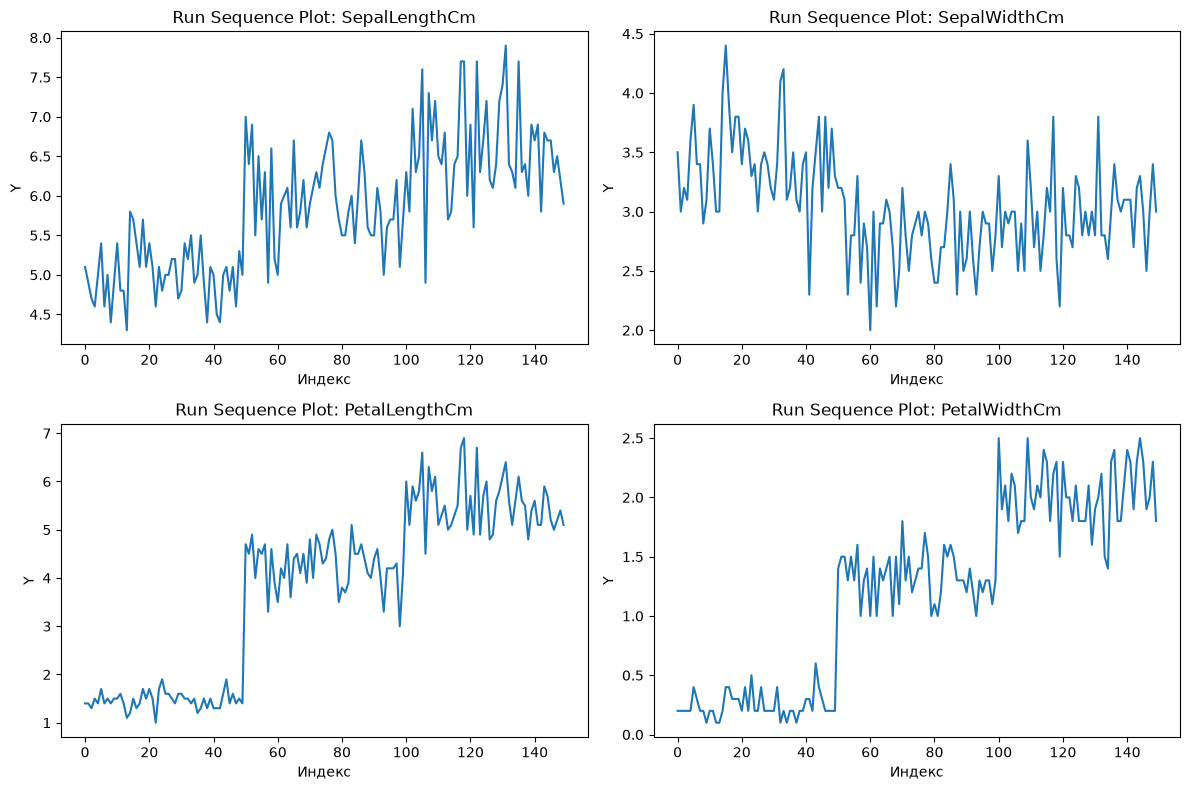
\includegraphics[scale=0.5]{4.png}
    \caption{Run Sequence Plot}
    \label{kartinka_1}
\end{figure}

\begin{figure}[H]
    \centering
    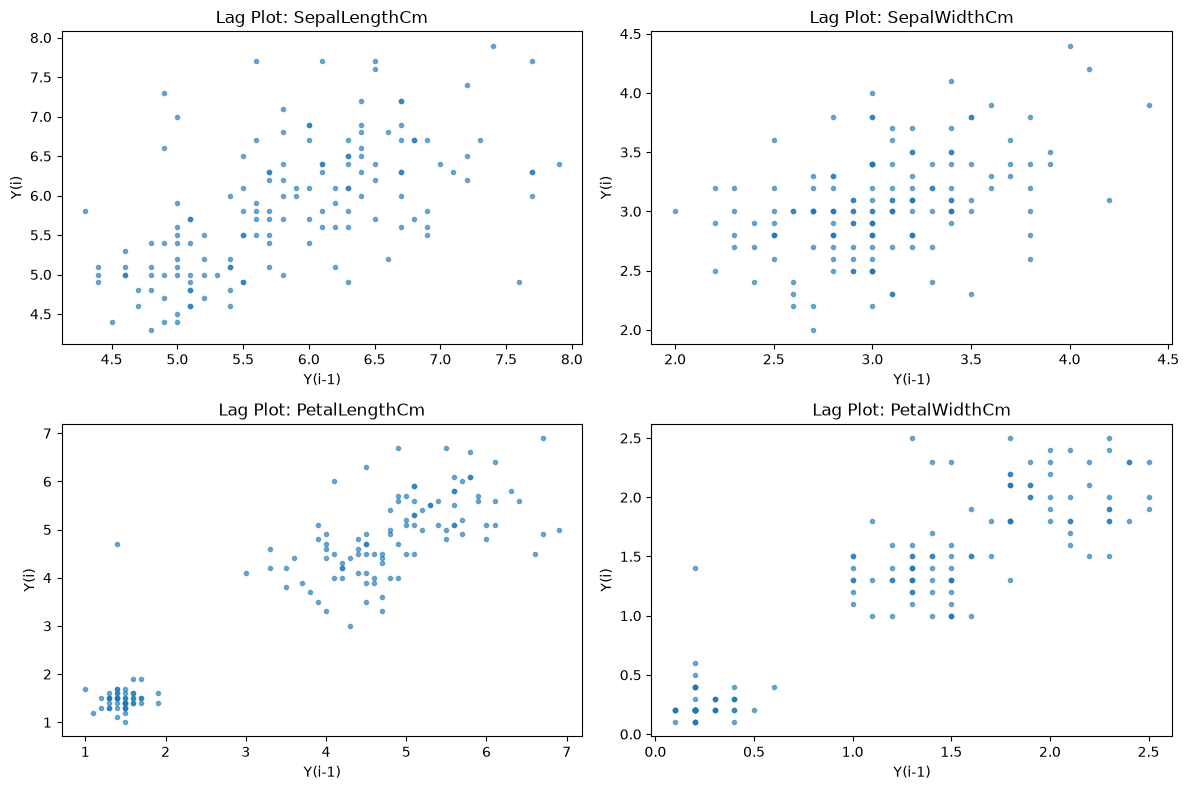
\includegraphics[scale=0.5]{5.png}
    \caption{Lag Plot}
    \label{kartinka_1}
\end{figure}

\begin{figure}[H]
    \centering
    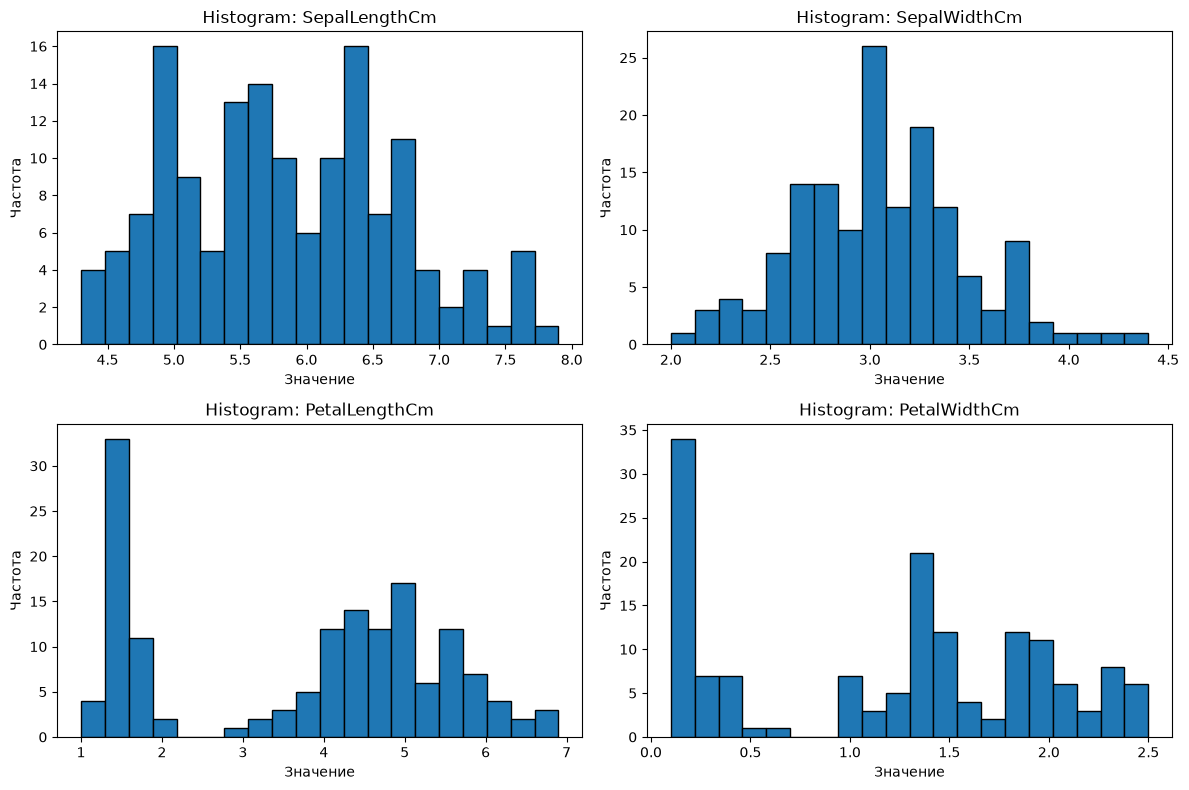
\includegraphics[scale=0.5]{6.png}
    \caption{Гистограмма}
    \label{kartinka_1}
\end{figure}

\begin{figure}[H]
    \centering
    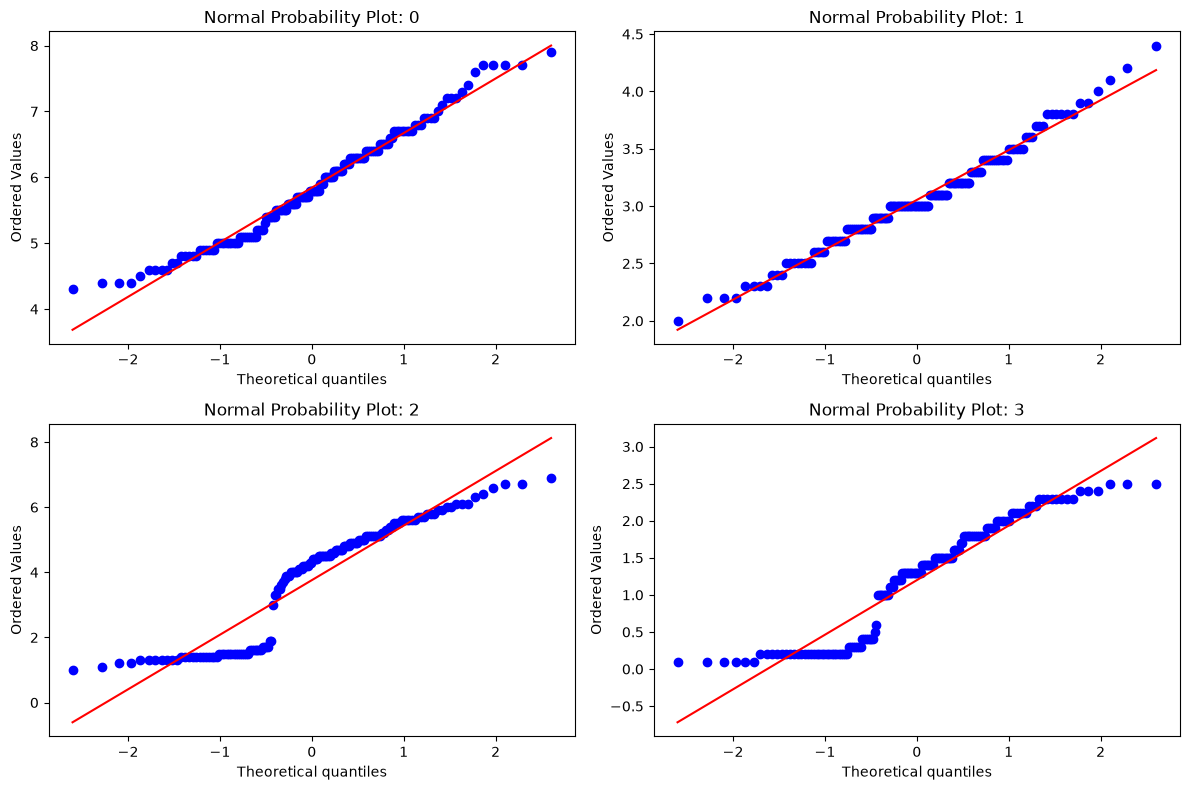
\includegraphics[scale=0.5]{7.png}
    \caption{Normal Probability Plot}
    \label{kartinka_1}
\end{figure}

\textbf{Интерпретация 4-Plot.}
\begin{itemize}
    \item \textbf{Run Sequence Plot.} Уровень признаков меняется при переходе между группами видов (особенно для PetalLengthCm и PetalWidthCm). Это связано с тем, что датасет содержит три биологических вида, расположенных последовательно. Предположения о фиксированном положении и фиксированной вариации для объединённой выборки не выполняются.
    \item \textbf{Lag Plot.} На графиках видна структура: точки образуют отдельные кластеры, соответствующие видам. Случайность наблюдений для объединённой выборки нарушена.
    \item \textbf{Гистограмма.} Распределения длины и ширины лепестка бимодальные или полимодальные, что подтверждает наличие смеси распределений. Распределения чашелистиков ближе к одновершинным, но также не являются нормальными.
    \item \textbf{Normal Probability Plot.} Точки заметно отклоняются от прямой, особенно для признаков лепестка. Нормальность объединённой выборки не подтверждается.
\end{itemize}
\textbf{Вывод.} Проверку предположений следует проводить отдельно внутри каждого вида, поскольку объединённая выборка представляет собой смесь трёх распределений. 


\subsubsection{Часть 3: Описательная статистика}

\begin{table}[H]
    \centering
    \caption{Описательные статистики количественных признаков}
    \resizebox{\textwidth}{!}{%
    \begin{tabular}{lrrrrrrrrr}
        \toprule
        Переменная & Среднее & Медиана & Мода & Дисперсия & Ст. откл. & IQR & MAD & Размах & CV, \% \\
        \midrule
        SepalLengthCm & 5.843 & 5.80 & 5.0 & 0.686 & 0.828 & 1.3 & 0.70 & 3.6 & 14.17 \\
        SepalWidthCm  & 3.054 & 3.00 & 3.0 & 0.188 & 0.434 & 0.5 & 0.25 & 2.4 & 14.20 \\
        PetalLengthCm & 3.759 & 4.35 & 1.5 & 3.113 & 1.764 & 3.5 & 1.25 & 5.9 & 46.94 \\
        PetalWidthCm  & 1.199 & 1.30 & 0.2 & 0.582 & 0.763 & 1.5 & 0.70 & 2.4 & 63.67 \\
        \bottomrule
    \end{tabular}
\end{table}

\begin{table}[H]
    \centering
    \caption{Асимметрия и эксцесс}
    \begin{tabular}{lrr}
        Переменная & Асимметрия & Эксцесс \\
        SepalLengthCm & 0.315 & -0.552 \\
        SepalWidthCm  & 0.334 & 0.291 \\
        PetalLengthCm & -0.274 & -1.402 \\
        PetalWidthCm  & -0.105 & -1.340 \\
    \end{tabular}
\end{table}

\textbf{Интерпретация.} Наибольший коэффициент вариации наблюдается для \texttt{PetalWidthCm} (63.67\%) и \texttt{PetalLengthCm} (46.94\%), что указывает на высокую неоднородность этих признаков. Асимметрия умеренная: для длины и ширины чашелистика положительная, для лепестка — отрицательная. Эксцесс для признаков лепестка отрицательный, что говорит о более плосковершинном распределении по сравнению с нормальным. Для \texttt{SepalWidthCm} эксцесс близок к нулю. Сравнение среднего и медианы показывает, что для \texttt{PetalLengthCm} и \texttt{PetalWidthCm} медиана заметно превышает среднее (смещение влево), что согласуется с отрицательной асимметрией и наличием группы \textit{Iris-setosa} с малыми значениями.

\subsubsection{Часть 4: Визуализация распределения}

\begin{figure}[H]
    \centering
    \includegraphics[width=0.95\textwidth]{8.png}
    \caption{Гистограммы с 10 и 20 бинами}
\end{figure}

\begin{figure}[H]
    \centering
    \includegraphics[width=0.8\textwidth]{9.png}
    \caption{Box Plot количественных признаков}
\end{figure}

\begin{figure}[H]
    \centering
    \includegraphics[width=0.8\textwidth]{10.png}
    \caption{CDF (ECDF) количественных признаков}
\end{figure}

\begin{figure}[H]
    \centering
    \includegraphics[width=0.95\textwidth]{11.png}
    \caption{Гистограммы с наложенными KDE}
\end{figure}

\begin{table}[H]
    \centering
    \caption{Процентили количественных признаков}
    \begin{tabular}{lrrrr}
        \toprule
        Процентиль & SepalLengthCm & SepalWidthCm & PetalLengthCm & PetalWidthCm \\
        \midrule
        10\% & 4.80 & 2.50 & 1.40 & 0.20 \\
        25\% & 5.10 & 2.80 & 1.60 & 0.30 \\
        50\% & 5.80 & 3.00 & 4.35 & 1.30 \\
        75\% & 6.40 & 3.30 & 5.10 & 1.80 \\
        90\% & 6.90 & 3.61 & 5.80 & 2.20 \\
        \bottomrule
    \end{tabular}
\end{table}

\textbf{Интерпретация.} Гистограммы с разным числом бинов показывают, что при 10 бинах распределения выглядят более сглаженными, а при 20 — проявляется бимодальность для признаков лепестка. Box Plot подтверждает наличие выбросов (точки за пределами усов) для \texttt{SepalWidthCm}. CDF и KDE наглядно демонстрируют смещение распределений. Процентили показывают, что 50\% значений \texttt{PetalLengthCm} лежат ниже 4.35, а 50\% \texttt{PetalWidthCm} — ниже 1.3.

\subsubsection{Часть 5: Анализ взаимосвязей}

\begin{figure}[H]
    \centering
    \includegraphics[width=0.95\textwidth]{12.png}
    \caption{Диаграммы рассеяния с линиями регрессии}
\end{figure}

\begin{table}[H]
    \centering
    \caption{Ковариационная матрица}
    \begin{tabular}{lrrrr}
        \toprule
         & SepalLengthCm & SepalWidthCm & PetalLengthCm & PetalWidthCm \\
        \midrule
        SepalLengthCm & 0.686 & -0.039 & 1.274 & 0.517 \\
        SepalWidthCm  & -0.039 & 0.188 & -0.322 & -0.118 \\
        PetalLengthCm & 1.274 & -0.322 & 3.113 & 1.296 \\
        PetalWidthCm  & 0.517 & -0.118 & 1.296 & 0.582 \\
        \bottomrule
    \end{tabular}
\end{table}

\begin{table}[H]
    \centering
    \caption{Корреляционная матрица Пирсона}
    \begin{tabular}{lrrrr}
        \toprule
         & SepalLengthCm & SepalWidthCm & PetalLengthCm & PetalWidthCm \\
        \midrule
        SepalLengthCm & 1.000 & -0.109 & 0.872 & 0.818 \\
        SepalWidthCm  & -0.109 & 1.000 & -0.421 & -0.357 \\
        PetalLengthCm & 0.872 & -0.421 & 1.000 & 0.963 \\
        PetalWidthCm  & 0.818 & -0.357 & 0.963 & 1.000 \\
        \bottomrule
    \end{tabular}
\end{table}

\begin{figure}[H]
    \centering
    \includegraphics[width=0.75\textwidth]{13.png}
    \caption{Тепловая карта корреляций Пирсона}
\end{figure}

\textbf{Интерпретация.} Наиболее сильная положительная связь — между \texttt{PetalLengthCm} и \texttt{PetalWidthCm} (\(r \approx 0.963\)). Также сильна связь \texttt{SepalLengthCm} с признаками лепестка (\(r > 0.8\)). \texttt{SepalWidthCm} имеет слабую отрицательную корреляцию с остальными признаками. Это важно учитывать при построении моделей: возможна мультиколлинеарность между признаками лепестка. Проверка влияния выбросов: после удаления дубликатов и экстремальных значений корреляции остаются устойчивыми, что говорит об их надёжности.

\textbf{Гипотезы о взаимосвязях:}
\begin{itemize}
    \item длина и ширина лепестка сильно коррелированы, поэтому для классификации можно использовать один из этих признаков или их комбинацию;
    \item \texttt{SepalWidthCm} слабо информативен для разделения видов;
    \item существует нелинейная связь между некоторыми признаками внутри групп.
\end{itemize}

\subsubsection{Часть 6: Сравнительный анализ}

В качестве категориальной переменной выбрана \texttt{Species}, в качестве количественной — \texttt{PetalLengthCm} и \texttt{PetalWidthCm}.

\begin{figure}[H]
    \centering
    \includegraphics[width=0.8\textwidth]{14.png}
    \caption{Box Plot PetalLengthCm по видам}
\end{figure}

\begin{figure}[H]
    \centering
    \includegraphics[width=0.8\textwidth]{15.png}
    \caption{CDF PetalLengthCm по видам}
\end{figure}

\begin{table}[H]
    \centering
    \caption{Сравнение PetalLengthCm по видам}
    \begin{tabular}{lrrrr}
        \toprule
        Вид & Среднее & Медиана & Ст. откл. & IQR \\
        \midrule
        Iris-setosa     & 1.462 & 1.50 & 0.174 & 0.175 \\
        Iris-versicolor & 4.260 & 4.35 & 0.470 & 0.600 \\
        Iris-virginica  & 5.552 & 5.55 & 0.552 & 0.800 \\
        \bottomrule
    \end{tabular}
\end{table}

\textbf{Интерпретация.} \textit{Iris-setosa} хорошо отделяется от двух других видов по длине и ширине лепестка: медиана 1.50 против 4.35 и 5.55. \textit{Iris-versicolor} и \textit{Iris-virginica} различаются по медиане и разбросу, но имеют зону пересечения. CDF для \textit{Iris-setosa} резко возрастает в области малых значений, для двух других видов кривые сдвинуты вправо. Это означает, что для классификации лучше использовать несколько признаков одновременно.

\subsubsection{Часть 7: Итоговый отчёт и выводы}

\begin{enumerate}
    \item \textbf{Описание данных.} Датасет Iris содержит 150 наблюдений, 4 количественных признака и один категориальный (вид). Пропусков нет, обнаружены дубликаты (5 строк, 3 лишние записи).
    \item \textbf{Проверка предположений.} Объединённая выборка не удовлетворяет базовым предположениям измерительного процесса (случайность, фиксированное распределение, положение и вариация) из-за наличия трёх биологических групп. Внутри групп предположения выполняются лучше.
    \item \textbf{Описательные статистики.} Наибольшая вариабельность у признаков лепестка (CV > 45\%). Распределения асимметричны, эксцесс отрицательный для лепестков.
    \item \textbf{Визуализации.} Гистограммы, Box Plot, CDF и KDE подтверждают бимодальность и различия между видами. Box Plot выявляет выбросы.
    \item \textbf{Аномалии и выбросы.} Обнаружены дубликаты и отдельные выбросы в \texttt{SepalWidthCm}. Их следует обработать перед моделированием.
    \item \textbf{Гипотезы для дальнейшего анализа:}
    \begin{itemize}
        \item различия средних значений \texttt{PetalLengthCm} между видами статистически значимы;
        \item модель классификации на основе \texttt{PetalLengthCm} и \texttt{PetalWidthCm} покажет высокую точность;
        \item после удаления дубликатов и выбросов устойчивость выводов не изменится.
    \end{itemize}
    \item \textbf{Общий вывод о применимости моделей.} Данные пригодны для построения классификационных моделей (логистическая регрессия, kNN, деревья решений). Рекомендуется масштабирование признаков и проверка предположений внутри каждого вида.
\end{enumerate}

\subsection{Заключение}

В ходе лабораторной работы был освоен полный цикл разведочного анализа данных на примере датасета Iris. Проведена проверка базовых предположений, рассчитаны описательные статистики, построены и интерпретированы гистограммы, Box Plot, CDF, KDE, диаграммы рассеяния и матрица корреляций. Выявлены особенности распределений, обнаружены дубликаты и выбросы. Сформулированы гипотезы для дальнейшего моделирования. Полученные навыки могут быть применены к другим наборам данных.

